\documentclass{beamer}
\usetheme{metropolis}           % Use metropolis theme

\usepackage[T2A]{fontenc}
\usepackage[utf8]{inputenc}
\usepackage[english, main=russian]{babel}

\usepackage{listingsutf8}
\usepackage[ruled]{algorithm}
\usepackage{algorithmicx}
\usepackage[noend]{algpseudocode}
\usepackage{amsmath}
\usepackage{caption} 
\usepackage{graphicx}
\usepackage{subcaption}
\usepackage{float}
\usepackage[newfloat]{minted}
\usepackage{longtable}                              % Длинные таблицы
\usepackage{multirow,makecell,array}                % Улучшенное форматирование таблиц
\usepackage{booktabs}
\usepackage{tabularx}

\floatname{algorithm}{Листинг}
\renewcommand{\algorithmname}{Листинг}

\title{Использование колоночных баз данных для хранения данных журналирования}
% \date{\today}
\author{Киселев Кирилл}
\author[me]{Выполнил: Киселев Кирилл ИУ9-61Б\\[1mm]Руководитель: Цалкович П.А.}
% \thanks
% \institute{МГТУ им. Н.Э. Баумана}
\begin{document}
\maketitle

\begin{frame}{Цели и задачи}
	\metroset{block=fill}
	\begin{alertblock}{Цель}
		Реализовать приложение позволяющее собирать и сохранять данные журналов приложений.
	\end{alertblock}
	\begin{alertblock}{Задачи}
		\begin{itemize}
			\item Изучить возможности и преимущества колоночных СУБД;
			\item Разработать приложение для сбора и сохранения лог-сообщений.
			\item Протестировать производительность итогового решения;
		\end{itemize}
	\end{alertblock}
\end{frame}


\begin{frame}{Журналирование}
	\metroset{block=fill}
	\begin{alertblock}{Где используются данные журналов}
		\begin{itemize}
			\item Обеспечение подотчётности;
			\item Диагностика проблем;
			\item Мониторинг;
		\end{itemize}
	\end{alertblock}
\end{frame}


\begin{frame}{Журналирование}
	\begin{alertblock}{Проблемы хранения данных журналов}
		\begin{itemize}
			\item Производительность традиционных СУБД;
			\item Необходимость масштабирования;
			\item Затруднительный анализ;
		\end{itemize}
	\end{alertblock}
\end{frame}


\begin{frame}{NoSQL}

	\begin{figure}
		\begin{minipage}{0.36\textwidth}
			\begin{alertblock}{Категории NoSQL}
				\begin{enumerate}
					\item Ключ-значение;
					\item Документо-ориентированные;
					\item Колоночные;
					\item Графовые.
				\end{enumerate}
			\end{alertblock}
		\end{minipage}
		\hfill
		\begin{minipage}{0.62\textwidth}
			\centering
			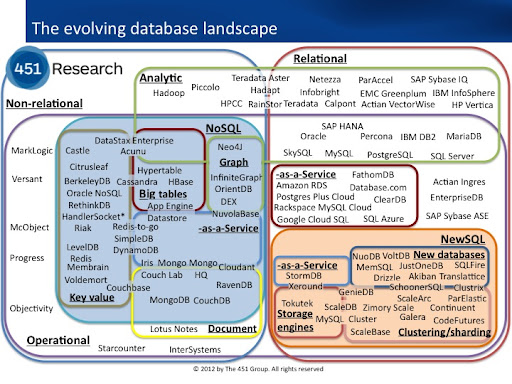
\includegraphics[width=\linewidth]{./imgs/dblandscape.jpg}
			\caption{Соотношение категорий СУБД}
		\end{minipage}
	\end{figure}

\end{frame}

\begin{frame}{Колоночные СУБД}
	\begin{figure}[H]
		\centering
		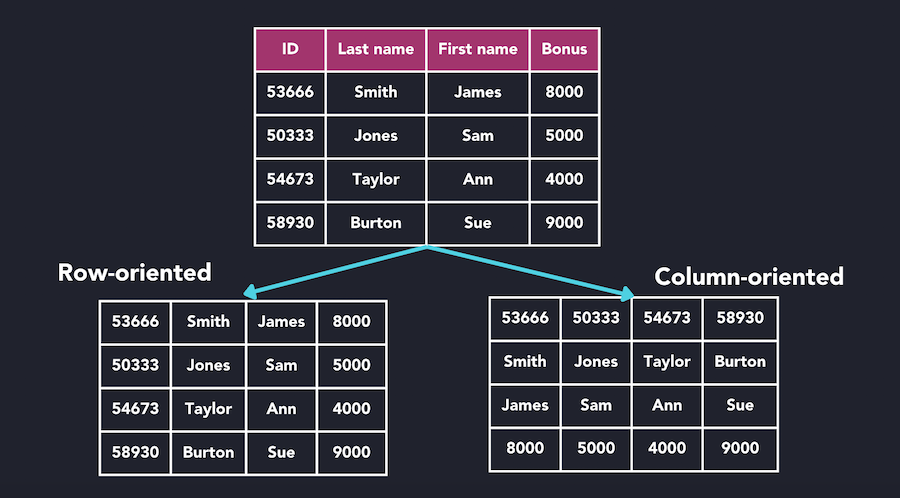
\includegraphics[width=.8\linewidth]{./imgs/columnar-database.png}
		\caption{Хранение данных в колоночных СУБД}
	\end{figure}
\end{frame}

\begin{frame}{Колоночные СУБД }

	\metroset{block=fill}
	\begin{alertblock}{Основные преимущества:}
		\begin{itemize}
			\item Высокая степень сжатия данных;
			\item Скорость операций агрегации;
			\item Гибкость схемы данных;
		\end{itemize}
	\end{alertblock}
\end{frame}

\begin{frame}{Колоночные СУБД}
	\metroset{block=fill}
	\begin{alertblock}{Популярные представители:}
		\begin{itemize}
			\item Apache Cassandra;
			\item ClickHouse;
			\item Google Bigtable;
			\item Apache HBase;
			\item Vertica;
		\end{itemize}
	\end{alertblock}
\end{frame}

\begin{frame}{СУБД ClickHouse}
	\begin{itemize}
	\end{itemize}
	\begin{figure}[H]
		\centering
		\begin{minipage}[t]{.9\textwidth}
			\centering
			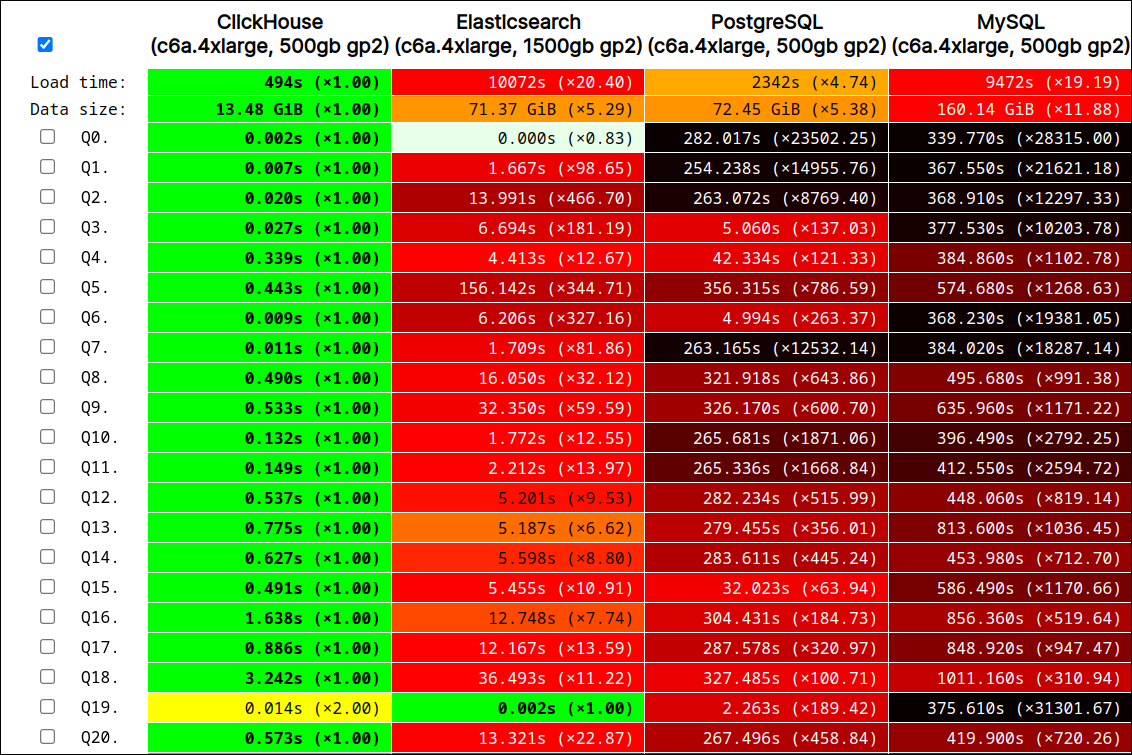
\includegraphics[width=.9\textwidth]{./imgs/clickbench.png}
		\end{minipage}
		\caption{Сравнение производительности ClickHouse c другими СУБД}
	\end{figure}
\end{frame}

\begin{frame}{Разработка Приложения}
	\begin{figure}[H]
		\centering
		\begin{minipage}[t]{1.2\textwidth}
			\centering
			
\includegraphics[width=.7\textwidth]{./imgs/appscheme.png}
		\end{minipage}
		\caption{Архитектура Приложения}
	\end{figure}
\end{frame}


\begin{frame}{Реализация приложения}
	\begin{alertblock}{Модули приложения}
		\begin{itemize}
			\item Интерфейс взаимодействия: REST API;
			\item Модуль чтения сообщений Apache Kafka;
			\item Модуль взаимодействия с СУБД ClickHouse.
		\end{itemize}
	\end{alertblock}
\end{frame}

\begin{frame}{Интерфейс взаимодействия}
	\begin{figure}[H]
		\centering
		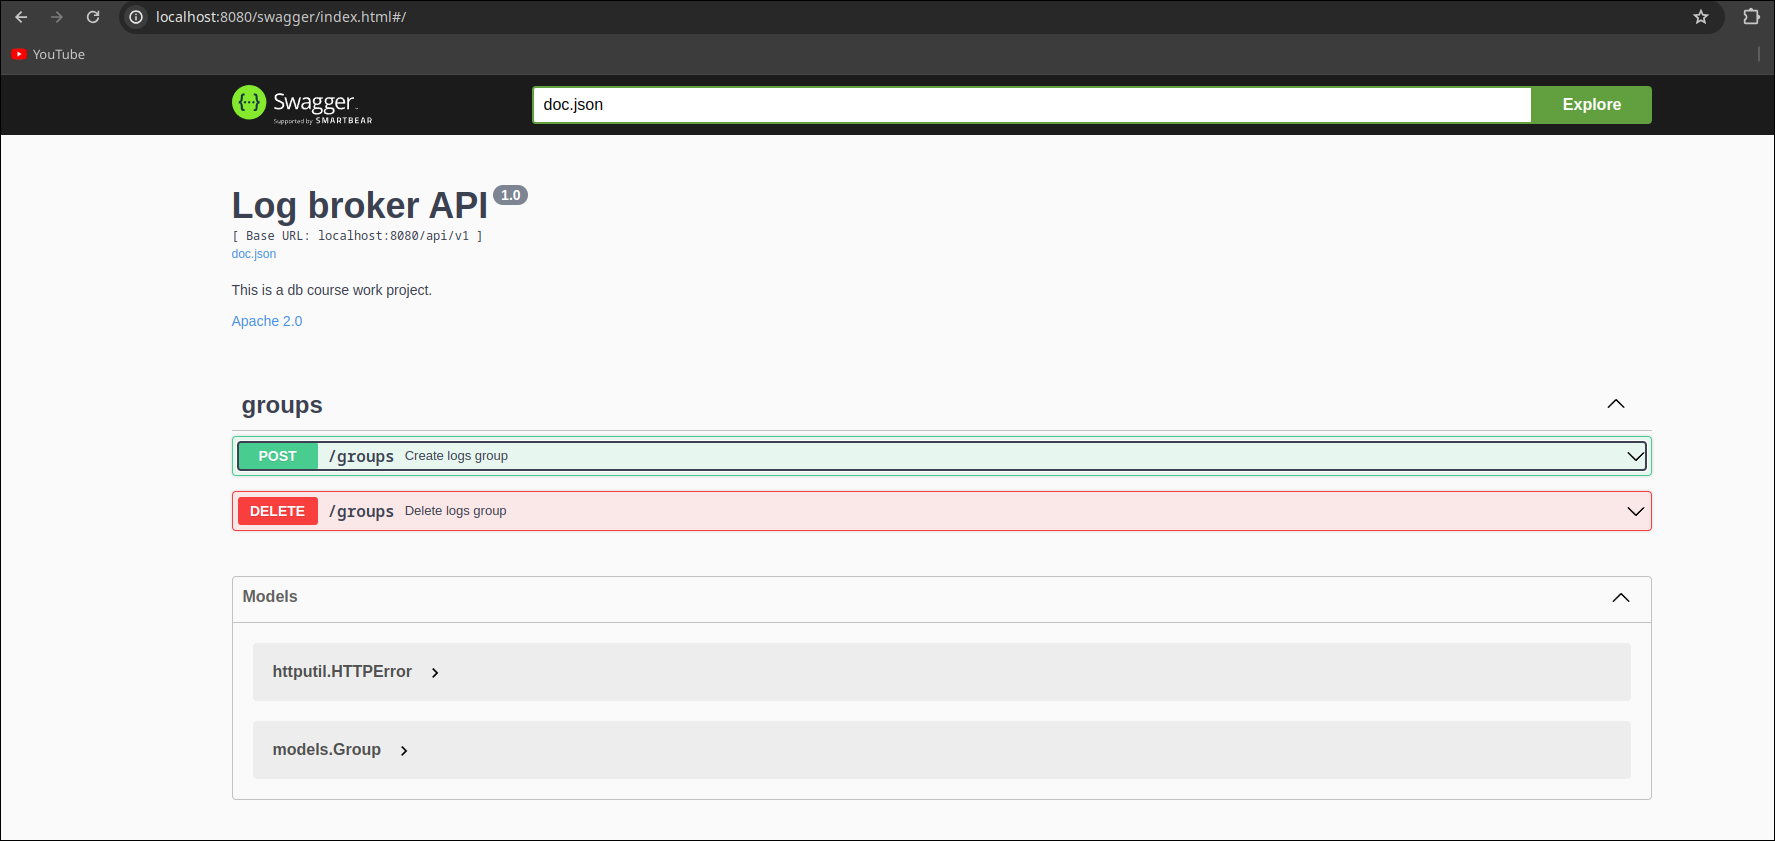
\includegraphics[width=.9\textwidth]{./imgs/swagger.png}
    \caption{REST API в формате OpenAPI(Swagger)}
	\end{figure}

\end{frame}

\begin{frame}{Интеграция с Apache Kafka}
	\metroset{block=fill}
  \begin{alertblock}{Библиотека Sarama}
    \item Нативная библиотека;
    \item Активное сообщество;
    \item Подробная документация с примерами использования;
  \end{alertblock}
\end{frame}

\begin{frame}{Интеграция с ClickHouse}
  \begin{listing}[H]
		\caption{Структура для взаимодействия с ClickHouse}
		\inputminted[style=bw, frame=single,fontsize=\small, linenos=true, xleftmargin = 1.5em, breaklines=true]{golang}{./listings/click_repo.go}
	\end{listing}
\end{frame}

\begin{frame}{Интеграция с ClickHouse}
  \begin{listing}[H]
		\caption{Множественная вставка в ClickHouse}
		\inputminted[style=bw, frame=single,fontsize=\small, linenos=true, xleftmargin = 1.5em, breaklines=true]{golang}{./listings/bulk_insert_body.go}
	\end{listing}
\end{frame}

\begin{frame}{Тестирование}
	\begin{table}[H]
		\caption{\centering Результаты тестирования приложения}
		\centering
		\begin{tabularx}{\textwidth}{|X|X|X|l|}
			\hline
			\textbf{Размер вставки} & \textbf{Среднее время вставки, мс} & \textbf{Медианное время вставки, мс} & \textbf{Сумарное время(сек)} \\ \hline
			100                     & 4.313                              & 4.078                                & 3.769                        \\ \hline
			250                     & 4.531                              & 4.274                                & 1.776                        \\ \hline
			500                     & 5.740                              & 5.604                                & 1.148                        \\ \hline
			1000                    & 9.394                              & 8.915                                & 0.940                        \\ \hline
			5000                    & 33.130                             & 32.746                               & 0.663                        \\ \hline
			10000                   & 67.990                             & 60.419                               & 0.680                        \\ \hline
			20000                   & 133.698                            & 119.987                              & 0.668                        \\ \hline
		\end{tabularx}
	\end{table}
\end{frame}


\begin{frame}{Визуализация данных}
	\begin{listing}[H]
		\caption{Конфигурация Fluent-Bit}
		\inputminted[style=bw, frame=single,fontsize = \small, linenos=true, xleftmargin = 1.5em, breaklines=true]{sql}{./listings/codes.sql}
	\end{listing}
	\begin{figure}[H]
		\centering
		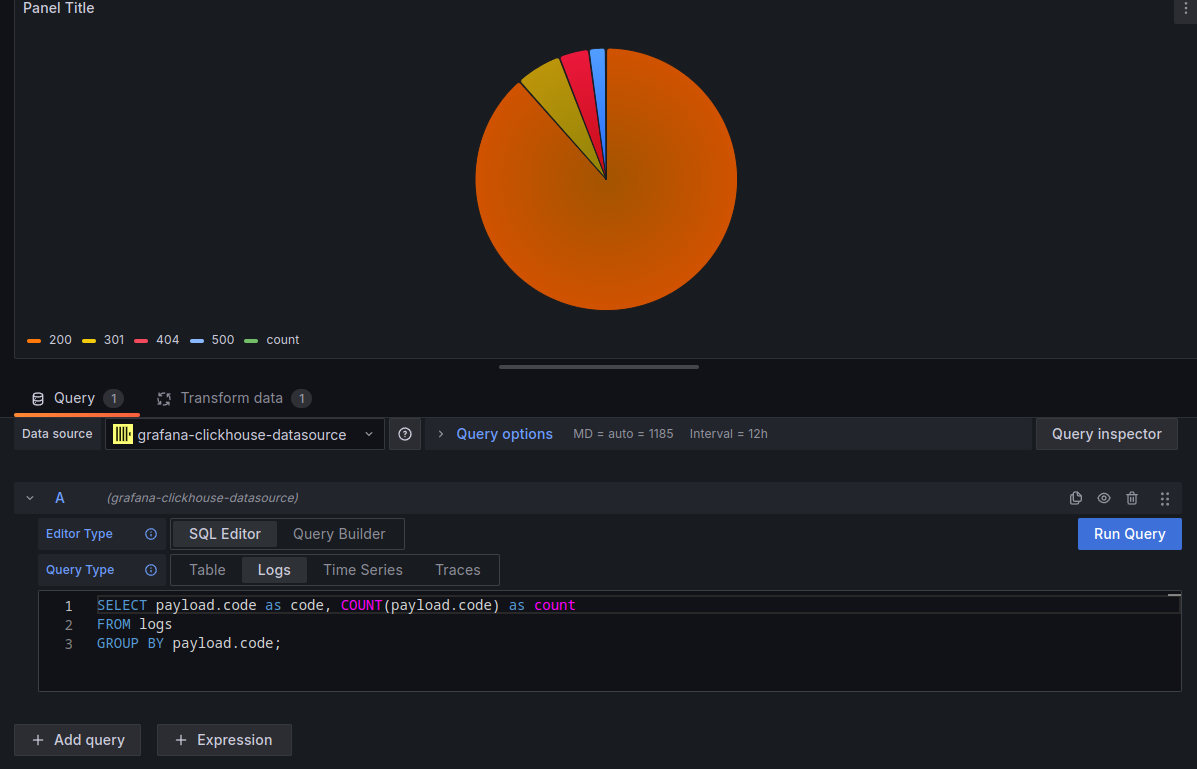
\includegraphics[width=.5\textwidth]{./imgs/nginx_grafana_status_codes.png}
		\caption{Визуализация распределения кодов ответов на основе сообщений журнала}
	\end{figure}

\end{frame}

\begin{frame}{Визуализация данных}
	\begin{listing}[H]
		\caption{Конфигурация Fluent-Bit}
		\inputminted[style=bw, frame=single,fontsize = \small, linenos=true, xleftmargin = 1.5em, breaklines=true]{sql}{./listings/grafana_nginx_requests.sql}
	\end{listing}

	\begin{figure}[H]
		\centering
		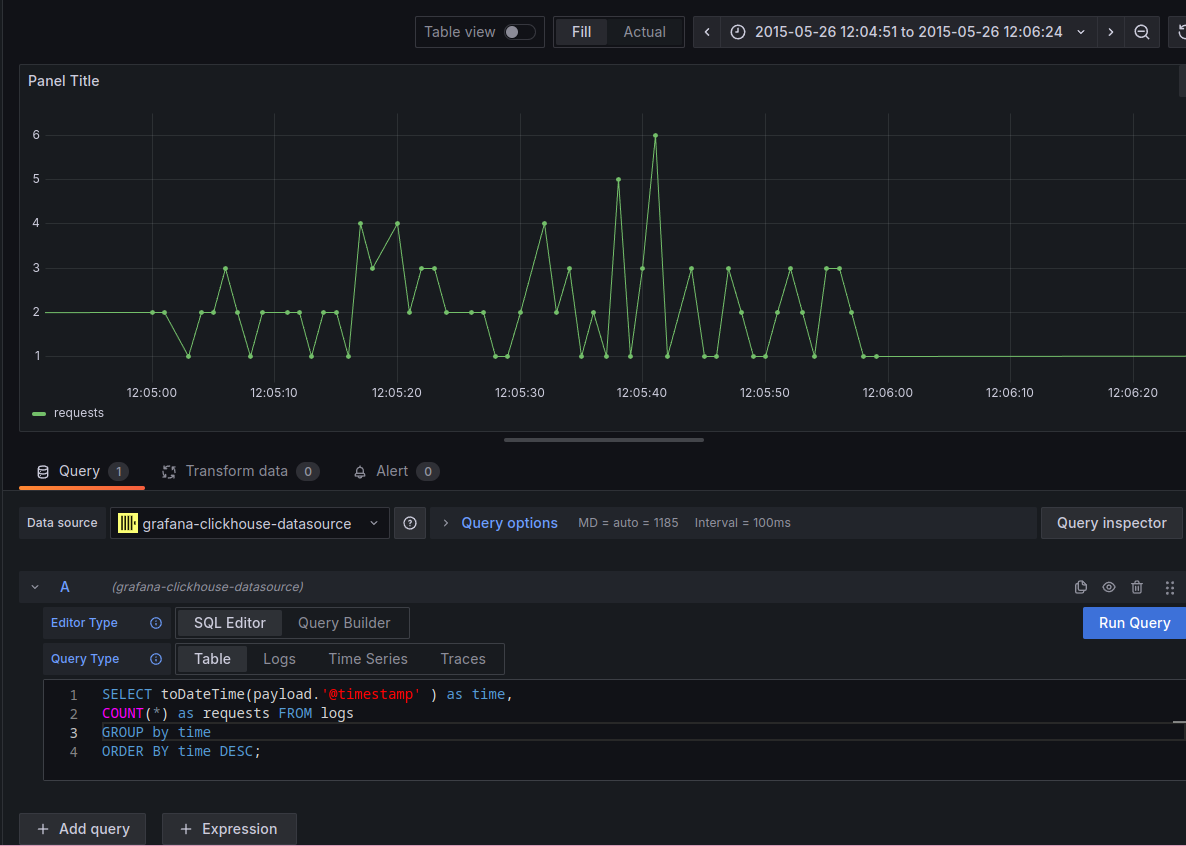
\includegraphics[width=.5\textwidth]{./imgs/nginx_grafana_requests.png}
		\caption{Визуализация частоты запросов на основе сообщений журнала}
	\end{figure}

\end{frame}

\begin{frame}{Визуализация данных}
	\begin{listing}[H]
		\caption{Получение квантилей в ClickHouse}
		\inputminted[style=bw, frame=single,fontsize = \small, linenos=true, xleftmargin = 1.5em, breaklines=true]{sql}{./listings/quantiles.sql}
	\end{listing}

	\begin{figure}[H]
		\centering
		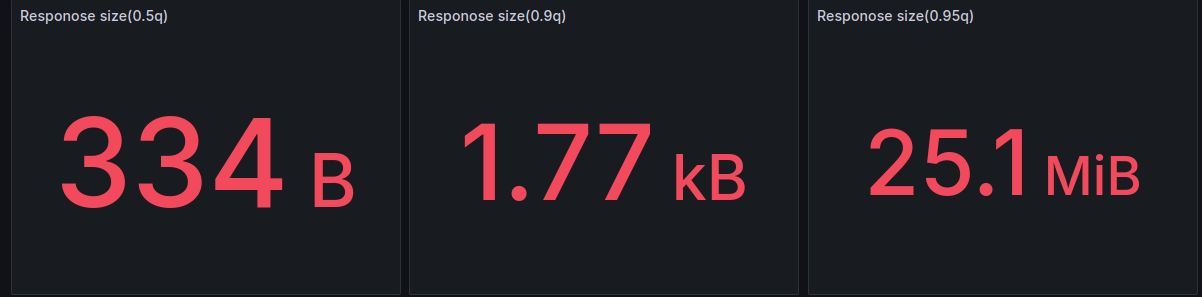
\includegraphics[width=.7\textwidth]{./imgs/nginx_grafana_size_quantilie.png}
		\caption{Квантили размеров ответов веб-сервера Nginx}
	\end{figure}
\end{frame}


\begin{frame}{Заключение}
	\begin{alertblock}{Возможные улучшения}
		\begin{itemize}
			\item Разработка Web-интерфейса;
			\item Расширение API;
			\item Покрытие кода модульными тестами;
		\end{itemize}
	\end{alertblock}
\end{frame}

\begin{frame}{Заключение}
	В ходе разработки были получены следующие навыки:
	\begin{itemize}
		\item Настройка и эксплуатация СУБД ClickHouse;
		\item Разработка на языке Golang;
		\item Использование брокера сообщений Apache Kafka для повышения доступности приложений;
		\item Визуализации данных СУБД ClickHouse в инструменте Grafana.
	\end{itemize}
\end{frame}


\end{document}
